Intrusive magmatism  is a major  process at  the scale of  a planetary
body and, most  likely, determinant in the evolution  of a terrestrial
crust. However,  it takes  place deep beneath  the surface  and remain
difficult  to study  without  a proper  model  for magmatic  intrusion
emplacement.  The objective of this thesis was two-fold: to characterize the
dynamics of  a cooling  magmatic intrusion  and to  shed light  on the
origin of floor-fractured craters. 

\section*{Dynamics of shallow magmatic intrusions.}

\subsection*{Summary}
\label{sec:summary}

Intermediate-scaled shallow magmatic intrusions are the building block
of      larger      plutons      intruded     into      the      crust
\citep{Petford:2000cc,Glazner:2004gv}.  We show in Chapter \ref{chap1}
that  the topographic  deformation  that could  be  caused by  shallow
intrusions can  be constrained by observations  of planetary surfaces;
that  is, volume,  shape and  other  dimensions of  intrusions can  be
quantified. These  observations have  been previously  used to  draw a
first view of their formation.  However, they must be linked to models
of magma  intrusion dynamics in  order to provide insights  into magma
physical properties and injection rate.

\citet{Michaut:2011kg}  provides  a  consistent $2D$  model  for  such
elastic-plated  gravity current  intrusions  which  directly link  the
observed  deformations  to  physical  parameters of  the  magmas.   In
particular, depending mainly  on the injection rate  and the intrusion
depth, two regimes of propagation  are identified and characterized by
specific morphologies and scaling  laws for intrusion thickness versus
length and time.   In Chapter \ref{chap2}, we develop the  model in an
axisymmetric  geometry  and  compare  the  model  predictions  to  the
morphology  of several  terrestrial shallow  magmatic intrusions.   We
show that  laccoliths and  low-slope lunar  domes are  consistent with
their arrest in the early times bending regime. In addition, the model
predictions    are     consistent    across     different    planetary
settings. However, the absolute dimension of these magmatic intrusions
is  underestimated  by  the  model;  in  particular,  abnormally  high
viscosity are required to reconcile both observations and predictions.

To get  some insight in  the effective  flow viscosity, we  provide in
chapter \ref{C3-JFM}  and \ref{Heating} an  extension of the  model of
\citet{Michaut:2011kg}   that  accounts   for  the   cooling  of   the
elastic-plated gravity current.  We show that the coupling between the
temperature field and  the flow itself results  in important deviation
from the  isoviscous case. In  particular, in the bending  regime, the
effective flow viscosity is governed by the local thermal condition at
the tip of  the current; as the fluid is  cooling, the thermal anomaly
detaches  from  the  tip  and the  flow  effective  viscosity  rapidly
increases   to  stabilize   when   it  reaches   its  maximum   value.
Applications  to   terrestrial  laccoliths  indeed  show   that  their
dimensions are  in agreement  with their arrest  in the  third bending
phase.  A  phase diagram as a  function of the Peclet  number $Pe$ and
the viscosity  contrast $\nu$ is  provided which allows  to constrains
the parameters of the intrusions  given its composition.  We then show
that lunar intrusive domes have  probably been characterized by larger
injection rate  than on Earth,  though much smaller than  the effusion
rates estimated from the runnout distance of some lunar lava flows.

Available data for large mafic sills on Earth show less agreement with
the   model  prediction.    Indeed,   in   chapter  \ref{C3-JFM}   and
\ref{Heating}, we  show that  sills should  also behave  as isoviscous
gravity current when the thermal anomaly is small compared to the flow
itself, i.e.   in similar settings,  their thickness should tend  to a
constant. Therefore, the increase in thickness with diameter preserved
in the data might suggest that they stop instead in the second gravity
phase. However, the model lacking of a stopping criteria for the flow,
this  hypothesis  can not  be  tested  properly.  Indeed,  in  chapter
\ref{Heating}, we  proposed that  the entrance in  the third  phase of
both  regimes might  have  triggered the  arrest  of shallow  magmatic
intrusions.   However,  even  for   laccoliths,  we  have  shown  that
conduction cooling  alone is probably  not a sufficient  mechanism for
their arrest, neither on Earth, nor on the Moon. In the end, while the
cooling of  the intrusion has  allowed us to  predict the mean  in the
observations, a  complete picture  of the solution,  in regard  to the
final  radius and  thickness of  the intrusion  as a  function of  the
parameters of the problem (elasticity  and toughness of the host rock,
viscosity of the  magma, injection rate of the feeder  dyke, and depth
of emplacement), has yet not been obtained.

\subsection*{Perspectives}
\label{sec:perspectives}

We show  in Chapter  \ref{chap2} that  terrestrial laccoliths  are too
small  to  be  fractured-controlled.    In  chapter  \ref{C3-JFM}  and
\ref{Heating},  we show  that the  dynamics in  the bending  regime is
controlled by  the local condition at  the tip of the  current.  For a
sake of simplicity, we used a thin prewetting film at the tip to avoid
the requirement  of any boundary  condition at a genuine  front. While
this approach allowed us to get insights into the coupling between the
thermal structure and the flow itself, a more precise characterization
of   the  front   might   help  predict   the   final  morphology   of
laccoliths. Indeed, the large negative  pressure that developed at the
front might cause desolved gasses to  exsolve from the magma.  In that
case, the formation and the evolution of  a gap filled with gas at the
tip  of the  current  might  provide a  mechanism  for  the arrest  of
laccolith.    Along   with   the   prewetting   film   regularization,
\citet{Anonymous:QWXp_4JV} propose  a second  regularization condition
where the tip of the elastic-gravity  current consists of a lag region
filled   with    gas   at    constant   negative    pressure   (Figure
\ref{C7-Sketch}).   They show  that the  solution depends  on the  gas
pressure  in the  tip  region  in similar  fashion  that the  solution
depends  on  the prewetting  film  thickness  in Chapter  \ref{chap2},
\ref{C3-JFM} and \ref{Heating}.
\begin{figure}[htpb]
  \begin{center}
    \graphicspath{ {/Users/thorey/Documents/These/Manuscript/Figure/Chapter7/} }
    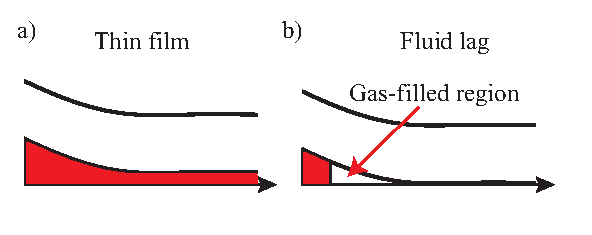
\includegraphics[scale=1.3]{Sketch.eps}
    \caption{Two different  regularization condition  at the  front of
      the current: a) thin prewetting film with thickness $h_f$ b) gas
      -filled region.}
    \label{C7-Sketch}
  \end{center}
\end{figure}

In  addition, the  difference for  the thickness  to radius  power law
relationship  are very  similar  for  both regularization  conditions,
i.e. $h_0\propto t^{9/23}$ and $R \propto t^{14/17}$


While the predicted  scaling laws are very similar in  both cases, the
complex dynamics of  the cooling gas-filled might  help understand the
arrest of such magmatic intrusions.



The weight of  the magma at the center may  eventually compensates for
the injection  rate at  the center. \citet{Michaut:2011kg}  have shown
that in that case, the intrusion enter a regime of lateral propagation
similar to the gravity current regime.



Indeed, for  a sake of simplicity,  we used a thin  prewetting film at
the  tip of  the  current to  avoid the  requirement  of any  boundary
condition at a genuine front.  In particular, this approach allowed us
to quantify  the effect  of cooling  to a  first order.   However, the
pressure closed to the advancing front becomes large and negative, and
might cause desolved gasses to exsolve  from the magma.  In that case,
the formation and the evolution of a gap filled with gas at the tip of
the current  might influence the  laccolith dynamics.  Along  with the
prewetting film  regularization, \citet{Anonymous:QWXp_4JV}  propose a
second regularization  condition where the tip  of the elastic-gravity
current consists of a lag region  filled with gas at constant negative
pressure in a cartesian geometry. While the predicted scaling laws are
very  similar in  both  cases,  the complex  dynamics  of the  cooling
gas-filled  might   help  understand  the  arrest   of  such  magmatic
intrusions.



\section*{Floor-fractured  craters and  their implication  in term  of
  lunar intrusive magmatism.}

About $200$ hundreds floor-fractured craters have been observed at the
surface  of   the  Moon.   Both  theoretical   model  predictions  and
gravitational   observations  confirms   their  link   with  intrusive
activity. 

Depression on the Earth have been shown to favor magma intrusion. 

%%% Local Variables:
%%% mode: latex
%%% TeX-master: "../main"
%%% End:

